% 第6章第3节：归一化拉普拉斯（度加权内积、对称归一化拉普拉斯、随机游走拉普拉斯、两种归一化的联系）。

\section{归一化拉普拉斯}
\label{sec:graph-normalized-laplacian}

组合拉普拉斯平等对待每个顶点上的数值。当各顶点的连接总量相差很大时，这种平等会带来偏差：改变连接多的顶点上的值，会同时牵动许多条边。本节先用度给长度加权，再经坐标缩放得到对称归一化拉普拉斯，然后从邻域平均得到随机游走拉普拉斯，最后说明二者的关系。

下面的公式要对加权度取倒数或倒数平方根，只对正度顶点有意义。记$V_+=\{i\in V:d_i>0\}$。度为零的顶点没有任何正权邻边，它在正权支撑图中是孤立点，下文称为支撑孤点；结构上它可能仍连着零权边。每个公式先在正度顶点上建立，再单独约定支撑孤点的处理。

\subsection{度加权内积}
\label{sec:graph-spec-degree-inner-product}

先看连接多少怎样影响能量。图~\ref{fig:graph-spec-degree-weighted-length}是单位权星图，中心连着三片叶，中心的度为$3$，叶的度为$1$。只在中心放一个单位值时，三条边都出现差$1$，能量为$3$；只在一片叶上放同样的单位值，只有一条边有差，能量为$1$。两个函数的欧氏长度都是$1$，能量却相差三倍。原因不在数值本身，而在中心连接更多：同样大小的改动，放在高度顶点上要被更多条边计入。

\begin{figure}[!htb]
  \centering
  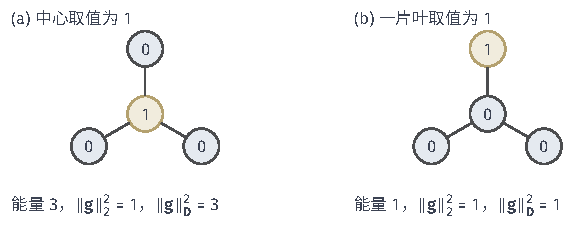
\includegraphics[width=97mm]{figures/01-basic-mathematics/04-graphs/tikz/c6-degree-weighted-length/figure.pdf}
  \caption{单位权星图上的两个单位脉冲，黄色顶点取值$1$，其余为$0$。(a)~中心的度为$3$，能量为$3$；(b)~叶的度为$1$，能量为$1$。两者的欧氏长度平方都是$1$，按度加权的长度平方分别为$3$和$1$，与能量成相同比例。}
  \label{fig:graph-spec-degree-weighted-length}
\end{figure}

如果在衡量函数大小时也把连接量计入，用$\sum_id_ig_i^2$代替$\sum_ig_i^2$，两个脉冲的长度平方就分别是$3$和$1$，能量与长度之比都等于$1$。这提示了一种新的内积：对定义在$V_+$上的函数，令
\begin{equation}
 \langle\bm g,\bm h\rangle_{\bm D}=\bm g^{\top}\bm D\bm h=\sum_{i\in V_+}d_ig_ih_i .
 \label{eq:graph-spec-degree-inner-product}
\end{equation}
在$V_+$上$\bm D$是正对角矩阵，因而对称正定，这正是第~\ref{sec:ls-weighted-inner-products}节的加权内积，称为\term{度加权内积}（degree-weighted inner product）。它与欧氏内积的区别只在于每个顶点的贡献乘以了该点的度。

加权内积可以换回普通内积，办法是缩放坐标。令$\bm f=\bm D^{1/2}\bm g$，即$f_i=\sqrt{d_i}\,g_i$，则
\[
 \lVert\bm f\rVert_2^2=\sum_id_ig_i^2=\bm g^{\top}\bm D\bm g=\lVert\bm g\rVert_{\bm D}^2 .
\]
在新坐标$\bm f$中，度加权长度就是欧氏长度，第三部分关于欧氏内积和对称矩阵的结论可以直接使用。含支撑孤点时，$\bm D$在整个$\mathbb R^n$上是奇异的：取$\bm g$为孤点$v$处的坐标向量$\bm e_v$，有$\bm g^{\top}\bm D\bm g=d_v=0$而$\bm g\neq\bm0$，正定性不成立。所以式~\eqref{eq:graph-spec-degree-inner-product}只在$V_+$上是内积，不能直接称为全空间的内积。

\subsection{对称归一化拉普拉斯}
\label{sec:graph-spec-symmetric-normalized}

先在全体顶点度为正的情形下推导。函数$\bm g$的能量是$\bm g^{\top}\bm L\bm g$，它的度加权长度平方是$\bm g^{\top}\bm D\bm g$。把坐标代换$\bm g=\bm D^{-1/2}\bm f$代入两者，得到
\[
 \frac{\bm g^{\top}\bm L\bm g}{\bm g^{\top}\bm D\bm g}
 =\frac{\bm f^{\top}\bm D^{-1/2}\bm L\bm D^{-1/2}\bm f}{\bm f^{\top}\bm f}.
\]
左端按度衡量的“每单位长度的能量”，在新坐标中变成了一个对称矩阵的普通Rayleigh商（定义~\ref{def:matrix-analysis-rayleigh-quotient}）。这个对称矩阵就是要找的算子。

\begin{definition}[对称归一化拉普拉斯]
\label{def:graph-spec-symmetric-normalized-laplacian}
设全体顶点的加权度为正，称
\begin{equation}
 \bm L_{\mathrm{sym}}=\bm D^{-1/2}\bm L\bm D^{-1/2}=\bm I-\bm D^{-1/2}\bm W\bm D^{-1/2}
 \label{eq:graph-spec-symmetric-normalized-laplacian}
\end{equation}
为\term{对称归一化拉普拉斯}（symmetric normalized Laplacian）。它的对角元为$1$，$(i,j)$位置的非对角元为$-w_{i,j}/\sqrt{d_id_j}$。
\end{definition}

逐边展开它的二次型，可以看出它比较的是什么。$\bm f^{\top}\bm L_{\mathrm{sym}}\bm f$就是$\bm g=\bm D^{-1/2}\bm f$的能量$\bm g^{\top}\bm L\bm g$，把$g_i=f_i/\sqrt{d_i}$代入式~\eqref{eq:graph-spec-dirichlet-energy}，得到
\begin{equation}
 \bm f^{\top}\bm L_{\mathrm{sym}}\bm f=\sum_{\{i,j\}\in E_+}w_{i,j}\left(\frac{f_i}{\sqrt{d_i}}-\frac{f_j}{\sqrt{d_j}}\right)^2\geq0 .
 \label{eq:graph-spec-normalized-energy}
\end{equation}
组合拉普拉斯比较的是相邻顶点的原值，$\bm L_{\mathrm{sym}}$比较的是先除以$\sqrt{d_i}$后的值。求和只经过正权边，而正权边的两个端点度都为正，分母不会出现零。

\paragraph{支撑孤点的约定}
有支撑孤点时，式~\eqref{eq:graph-spec-symmetric-normalized-laplacian}中的$\bm D^{-1/2}$无法按原样定义。约定$\bm D^{-1/2}$是对角矩阵，正度顶点处取$d_i^{-1/2}$，支撑孤点处取$0$，再用$\bm L_{\mathrm{sym}}=\bm D^{-1/2}\bm L\bm D^{-1/2}$定义。支撑孤点$v$在$\bm L$中的行和列本来全为零，在$\bm L_{\mathrm{sym}}$中也全为零，于是对角元$(\bm L_{\mathrm{sym}})_{v,v}=0$。在这一约定下，第二种写法$\bm I-\bm D^{-1/2}\bm W\bm D^{-1/2}$会在孤点处给出$1$，二者不再相同，所以有支撑孤点时只用第一种写法。

以单位权路径$1-2-3$外加孤立顶点$4$为例，度为$(1,2,1,0)$，按约定$\bm D^{-1/2}=\operatorname{diag}(1,\tfrac1{\sqrt2},1,0)$，于是
\[
 \bm L_{\mathrm{sym}}=\begin{bmatrix}1&-\tfrac1{\sqrt2}&0&0\\-\tfrac1{\sqrt2}&1&-\tfrac1{\sqrt2}&0\\0&-\tfrac1{\sqrt2}&1&0\\0&0&0&0\end{bmatrix}.
\]
它的第四行、第四列全为零。二次型~\eqref{eq:graph-spec-normalized-energy}只经过边$\{1,2\}$、$\{2,3\}$，与这个矩阵一致：$f_4$不出现在任何一项中。孤点给$\bm L_{\mathrm{sym}}$带来一个零特征值，它的谱留到第~\ref{sec:graph-spectrum-connectivity}节统一讨论。

\subsection{随机游走拉普拉斯}
\label{sec:graph-spec-random-walk-laplacian}

第~\ref{sec:graph-spec-neighborhood-aggregation}小节指出$\bm W\bm f$是加权和而不是平均。在正度顶点上把第$i$行除以$d_i$，就得到平均：
\[
 \bm P_{\mathrm{rw}}=\bm D^{-1}\bm W,\qquad
 (\bm P_{\mathrm{rw}}\bm f)_i=\sum_j\frac{w_{i,j}}{d_i}f_j .
\]
这里的下标与重编号用的置换矩阵$\bm P$相区别。$\bm P_{\mathrm{rw}}$每行的权非负且和为$1$，所以$(\bm P_{\mathrm{rw}}\bm f)_i$是邻居值的加权平均，介于邻居值的最小值与最大值之间。支撑孤点没有邻居可平均，约定$(\bm P_{\mathrm{rw}})_{v,v}=1$、该行其余元素为$0$，使孤点保持原值。在单位权三点路径上，$\bm P_{\mathrm{rw}}(3,1,2)^{\top}=(1,\tfrac52,1)^{\top}$：中间顶点得到两个邻居的平均$\tfrac52$，不再是和$5$。

本点值减去邻居平均，就得到第三个算子
\begin{equation}
 \bm L_{\mathrm{rw}}=\bm I-\bm P_{\mathrm{rw}} ,
 \label{eq:graph-spec-random-walk-laplacian}
\end{equation}
称为\term{随机游走拉普拉斯}（random-walk Laplacian）。在正度顶点的行上，$\bm L_{\mathrm{rw}}=\bm D^{-1}\bm L$，即$(\bm L_{\mathrm{rw}}\bm f)_i=(\bm L\bm f)_i/d_i$；支撑孤点的行全为零。上例中$\bm L_{\mathrm{rw}}(3,1,2)^{\top}=(2,-\tfrac32,1)^{\top}$，中间顶点的输出是$1-\tfrac52$。

名称中的“随机游走”来自对$w_{i,j}/d_i$的一种解释：把它看成从$i$出发下一步走到$j$的概率。完整的随机游走还需要随机序列和转移规则，它的稳态与收敛属于后续概率部分。本节只使用有限个非负权的加权平均，不涉及任何随机性或收敛结论。

\subsection{两种归一化的联系}
\label{sec:graph-spec-normalization-relations}

$\bm L_{\mathrm{sym}}$由坐标缩放得到，$\bm L_{\mathrm{rw}}$由邻域平均得到，两者其实是同一个作用的两种写法。在正度顶点上，
\[
 \bm D^{-1/2}\bm L_{\mathrm{sym}}\bm D^{1/2}=\bm D^{-1/2}\bm D^{-1/2}\bm L\bm D^{-1/2}\bm D^{1/2}=\bm D^{-1}\bm L=\bm L_{\mathrm{rw}} .
\]
所以二者相似（第~\ref{sec:ls-similarity}节），特征值相同，特征向量要经坐标转换：若$\bm L_{\mathrm{sym}}\bm x=\lambda\bm x$，则$\bm L_{\mathrm{rw}}(\bm D^{-1/2}\bm x)=\lambda\bm D^{-1/2}\bm x$。读法是：$\bm L_{\mathrm{rw}}$作用于原坐标$\bm g$，等于先换到$\bm f=\bm D^{1/2}\bm g$，用$\bm L_{\mathrm{sym}}$作用，再换回原坐标。

$\bm L_{\mathrm{rw}}$一般不对称。单位权三点路径上，它的$(1,2)$元是$-1$，$(2,1)$元是$-\tfrac12$。但它在度加权内积下自伴（第~\ref{sec:ls-adjoints}节）：由$\bm D\bm L_{\mathrm{rw}}=\bm L=\bm L^{\top}$，
\[
 \langle\bm L_{\mathrm{rw}}\bm g,\bm h\rangle_{\bm D}=\bm g^{\top}\bm L_{\mathrm{rw}}^{\top}\bm D\bm h=\bm g^{\top}\bm L\bm h=\langle\bm g,\bm L_{\mathrm{rw}}\bm h\rangle_{\bm D} .
\]
有支撑孤点时，这些关系都限制在正度顶点上成立。

\begin{figure}[!htb]
  \centering
  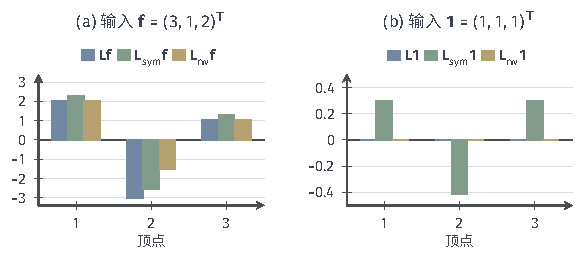
\includegraphics[width=98mm]{figures/01-basic-mathematics/04-graphs/tikz/c6-three-laplacians/figure.pdf}
  \caption{单位权三点路径（度为$1,2,1$）上三种拉普拉斯作用于同一向量。(a)~输入$(3,1,2)^{\top}$：$\bm L_{\mathrm{rw}}$把$\bm L$的输出逐点除以度，中间顶点从$-3$变为$-\tfrac32$；$\bm L_{\mathrm{sym}}$的输出约为$(2.29,-2.54,1.29)$。(b)~输入常量$\bm1$：$\bm L$与$\bm L_{\mathrm{rw}}$都给出零，$\bm L_{\mathrm{sym}}$不给出零。}
  \label{fig:graph-spec-three-laplacians}
\end{figure}

用一个度不相等的例子对照三个算子。单位权三点路径的度为$(1,2,1)$，图~\ref{fig:graph-spec-three-laplacians}(a)把它们作用于$\bm f=(3,1,2)^{\top}$：
\[
 \bm L\bm f=\begin{bmatrix}2\\-3\\1\end{bmatrix},\quad
 \bm L_{\mathrm{rw}}\bm f=\begin{bmatrix}2\\-\tfrac32\\1\end{bmatrix},\quad
 \bm L_{\mathrm{sym}}\bm f=\begin{bmatrix}3-\tfrac1{\sqrt2}\\1-\tfrac5{\sqrt2}\\2-\tfrac1{\sqrt2}\end{bmatrix}\approx\begin{bmatrix}2.29\\-2.54\\1.29\end{bmatrix}.
\]
$\bm L_{\mathrm{rw}}$只是把$\bm L$的输出逐点除以度，度为$1$的端点不变；$\bm L_{\mathrm{sym}}$则先把输入缩放成$\bm D^{-1/2}\bm f=(3,\tfrac1{\sqrt2},2)^{\top}$，再作用、再缩放，每个分量都变了。图~(b)换成常量输入$\bm1$：$\bm L\bm1=\bm L_{\mathrm{rw}}\bm1=\bm0$，而$\bm L_{\mathrm{sym}}\bm1=(1-\tfrac1{\sqrt2},1-\sqrt2,1-\tfrac1{\sqrt2})^{\top}\neq\bm0$。$\bm L_{\mathrm{sym}}$消去的是度缩放后的常量$\bm D^{1/2}\bm1=(1,\sqrt2,1)^{\top}$，因为$\bm L_{\mathrm{sym}}\bm D^{1/2}\bm1=\bm D^{-1/2}\bm L\bm1=\bm0$。

这个例子区分了三件不同的事。从$\bm L$到$\bm L_{\mathrm{rw}}$是改变算子：输出被逐点除以度，零向量不变，但输出的尺度变了。从$\bm L_{\mathrm{rw}}$到$\bm L_{\mathrm{sym}}$是改变坐标：同一个作用在$\bm g$坐标与$\bm f=\bm D^{1/2}\bm g$坐标中分别写成这两个矩阵。把欧氏内积换成度加权内积则是改变内积：$\bm L_{\mathrm{rw}}$在欧氏内积下不对称，在度加权内积下自伴。后面选取谱基、作谱划分时，都要先说明用的是哪个算子、哪种坐标。
